\documentclass[12pt, letterpaper]{article}
\usepackage{amsmath, amssymb, amsthm}
\usepackage{textcomp}
\usepackage{gensymb}
\usepackage{titlesec}
\usepackage{graphicx}

\graphicspath{{images/}}

\titleformat{\section}
[block]
{\Huge\bfseries\center}
{\thesection.\ }
{0pt}
{}

\titleformat{\subsection}
[block]
{\large\bfseries\center}
{\thesubsection\ }
{0pt}
{}

\titleformat{\subsubsection}
[block]
{\large\center}
{}
{0pt}
{}

\title{MATHD022: Discrete Mathematics}
\author{Connor Petri}
\date{Spring 2025}

\begin{document}

\maketitle
\pagebreak
\tableofcontents
\pagebreak

\section{The Language of Mathematics}
\hrulefill
\subsection{Variables}

\paragraph*{Definition} A \textbf{variable} is a symbol that is used as a placeholder when:
\begin{itemize}
    \item The quantity has one of more values, but is not known.
    \begin{itemize}
        \item For example: $2x^2 - x = 7$
    \end{itemize}
    \item The quantity represents \textbf{any element} from a given set.
    \begin{itemize}
        \item For example: The reciporical of any non-zero integer $n$ is $\frac{1}{n}$.
    \end{itemize}
\end{itemize}

\paragraph*{Writing Sentences using Variables}
We can rewrite the following sentences using variables:
\begin{itemize}
    \item Is there an integer $n$ that has a remainder of 2 when it is divided by 5?
    \begin{itemize}
        \item Is there an integer $n$ such that $n \% 5 = 2$?
    \end{itemize}
    \item The cube root of any negative real number is negative.
    \begin{itemize}
        \item For any real number $s$, if $s < 0$, then $\sqrt[3]{s} < 0$.
    \end{itemize}
\end{itemize}

\paragraph*{Types of Statements}
\begin{itemize}
    \item A \textbf{universal statement} is a statement that is true always true.
    \begin{itemize}
        \item For example: \textbf{All} positive numbers are greater than 0.
    \end{itemize}

    \item A \textbf{conditional statement} is a statement that is true if a certain condition is met.
    \begin{itemize}
        \item For example: \textbf{If} 378 is divisible by 18, \textbf{then} 378 is divisible by 6.
    \end{itemize}

    \item A \textbf{universal conditional statement} is a statement that is both conditional and universal.
    \begin{itemize}
        \item For example: \textbf{For all} animals $a$, if $a$ is a dog, \textbf{then} a is a mammal.
        \item As a universal statement: \textbf{For all} dogs $a$, $a$ is a mammal.
        \item As a conditional statement: \textbf{If} $a$ is a dog, \textbf{then} $a$ is a mammal.
    \end{itemize}

    \item An \textbf{existential statement} gives a property that is true for at least one thing.
    \begin{itemize}
        \item \textbf{There is} a prime number that is even.
    \end{itemize}

    \item A \textbf{universal existential statement} is a statement where the first part is universal and the second part is existential.
    \begin{itemize}
        \item \textbf{Every} real number \textbf{has} an additive inverse.
        \item \textbf{For all} real numbers $r$, \textbf{there is} an additive inverse $-r$.
        \item \textbf{For all} real numbers $r$, \textbf{there is} a real number $s$ such that $r + s = 0$.
    \end{itemize}

    \item An \textbf{existential universal statement} is a statement where the first part is existential and the second part is universal.
    \begin{itemize}
        \item \textbf{There is} a positive integer that is less than or equal to \textbf{every} positive integer.
        \item \textbf{There is} a positive intefer $m$ such that \textbf{every} positive integer is greater than or equal to $m$.
        \item \textbf{There is} a positive integer $m$ with the property that \textbf{for all} positive integers $n$, $m \leq n$.
    \end{itemize}
\end{itemize}
\subsection{Sets}
\paragraph*{Definition} 
A \textbf{set} is a collection of objects.

\paragraph*{Notation} 
\begin{itemize}
    \item $x \in S$: $x$ is an element of $S$.
    \item $x \notin S$: $x$ is not an element of $S$.
    \item $S = \{1,2,3, \dots\}$: is \textbf{set roster notation.}
\end{itemize}

\paragraph*{Axion of Extension}
A set is determined by what its elements are. Orders of elements or repeated elements can't be determine the set.\\
For example: $\{1,2,3\} = \{3,2,2,1,2,3,1\}$. There are 3 elements in both sets.

\paragraph*{Common Sets}
\begin{itemize}
    \item $\mathbb{R}$: the set of all real numbers.
    \item $\mathbb{Z}$: $\{\dots , -3,-2,-1,0,1,2,3,\dots\}$ the set of all integers.
    \item $\mathbb{N}$: $\{1,2,3,\dots\}$ the set of all natural numbers.
    \item $\mathbb{Q}$: the set of all rational numbers.
    \item $\emptyset = \{\}$: the empty set, or null set.
\end{itemize}

The null set is a subset of every set.

\paragraph*{Set Builder Notation}
Let $S$ denote a set and let $x\in S$ be and element in $S$. $P(x)$ is a property that some elements of $S$ satisfy.

\begin{center}
    $A = \{x\in S | P(x)\}$\\
    $A$ constains elements in $S$ such that (|) P(x) is true.
\end{center}

\pagebreak

\subsubsection*{Subsets}
\paragraph*{Definition}
Let $A$ and $B$ be sets. $A$ is a \textbf{subset} ($\subseteq$) of $B$ if every element of $A$ is also an element of $B$.\\

\paragraph*{Proper Subsets}
Let $A$ and $B$ be sets. $A$ is a \textbf{proper subset} ($\subset$) of $B$ if every element of $A$ is also an element of $B$, \textbf{and} 
there is at least one element in $B$ that is not in $A$.\\

\paragraph*{Example}
Let $A = \mathbb{Z^+}, B = \{n\in\mathbb{Z}|0\leq n\leq 100\}, and C = \{100,200,300,400,500\}$.
\begin{itemize}
    \item $B \subseteq A$ is false.
    \item $C \subset A$ is true.
    \item $C \subseteq B$ is false.
    \item $C \subseteq C$ is true.
\end{itemize}

\paragraph*{Cartesian Product of sets}
Let $A$ and $B$ be sets. The \textbf{Cartesian product} of $A$ and $B$, denoted $A\times B$, is the set of all ordered pairs $(a,b)$ such that $a\in A$ and $b\in B$.\\
\begin{equation*}
    A\times B = \{(a,b)|a\in A, b\in B\}
\end{equation*} 

\paragraph*{Example}
Let $A = \{1,2,3\}$ and $B = {u,v}$.
\begin{align*}
    A\times B &= \{(1,u),(1,v),(2,u),(2,v),(3,u),(3,v)\}\\
    A\times A &= \{(1,1),(1,2),(1,3),(2,1),(2,2),(2,3),(3,1),(3,2),(3,3)\}
\end{align*}
\subsection{Relations and Functions}

\paragraph*{Relations}
Let $A$ and $B$ be sets. A \textbf{relation} from $A$ to $B$ is a subset of the Cartesian product $A\times B$.\\
\begin{equation*}
    R \subseteq A\times B
\end{equation*}
\begin{itemize}
    \item If (x,y) $\in R$, we say that $x$ is related to $y$ by $R$, denoted as $xRy$.
    \item \textbf{A} is in the \textbf{domain} of \textbf{R}
    \item \textbf{B} is the \textbf{codomain} of \textbf{R}
\end{itemize}

\paragraph*{Example}
Let $A = \{1,2,3\}$ and $B = \{1,2\}$ and define a relation $R$ from $A$ to $B$ as follows:
\begin{align*}
    (x,y) &\in R \iff \frac{x+y}{2} \in \mathbb{Z}\\
    R = &\{(1,1), (1,2), (2,1), (2,2), (3,1)\}\\
        &\text{Domain of } R = \{1,2,3\}\\
        &\text{Codomain of } R = \{1,2\}\\
\end{align*}

\subsubsection*{Functions}
\paragraph*{Definition}
Let A and B be two sets. A function F from A to B is a relation with domain A and co-domain B that satisfies the following properties:
\begin{itemize}
    \item For every element $x \in A$, there is an element $y \in B$ such $(x,y) \in F$
    \item For every element $x \in A$,
\end{itemize}
\pagebreak
\paragraph*{Example}
Let  $A = \{2,4,6\}$ and $B = \{1,3,5\}$. Which of the relations defined below are functions from A to B?
\begin{itemize}
    \item $R = \{(2, 5), (4, 1), (4, 3), (6, 5)\}$
    \begin{itemize}
        \item Not a function because $4$ is related to $1$ and $3$. This is not a many-to-one relationship.
    \end{itemize}

    \item For all $(x.y) \in A \times B, (x,y) \in S \iff y = x + 1$
    \begin{itemize}
        \item $S = \{(2,3), (4,5)\}$ is a function from A to B.
    \end{itemize}

    \item $T = \{(2,5),(4,1),(6,1)\}$
    \begin{itemize}
        \item $T$ is a function from A to B as A has a many-to-one relationshop with B.
    \end{itemize}
\end{itemize}

\subsubsection*{Equivalent Functions}
Let A and B be two sets. Two functions $f$ and $g$ from A to B:
\begin{equation*}
    f = g \iff f(x) = g(x) \quad \forall \quad x \in A
\end{equation*}

\section{The Logic of Compound Statements}
\subsection{Logical Form and Equivalence}
\hrulefill
\subsubsection*{Arguments}

\paragraph*{Definition}
An arguement is a sequence of statements aimed at demonstrating the truth of an assertion.
\begin{itemize}
    \item The assertion at the end of the sequence is called the conclusion.
    \item The statements that support the conclusion are called premises.
    \item If the premises are true, the conclusion must also be true.
\end{itemize}

\paragraph*{Example}
\begin{itemize}
    \item If student A is a math major or student A is a computer science major,
    \item Then student A will take Discrete Math.
\end{itemize}

\subsubsection*{Logical Statements}
\paragraph*{Definition}
A logical statement is a declarative sentence that is either true or false, but not both.\\
\begin{itemize}
    \item Not $p$: \quad $\neg p$
    \item $p$ and/but $q$: \quad $p \land q$
    \item $p$ or $q$: \quad $p \lor q$
    \item Neither $p$ nor $q$: \quad $\neg p \land \neg q$
\end{itemize}

\paragraph*{Example}
h = healthy, w = wealthy, s = wise\\
\begin{itemize}
    \item John is healthy and wealthy but not wise. 
    \begin{itemize}
        \item $\quad (h \land w) \land \neg s$
    \end{itemize}
    \item John is neither wealthy nor wise, but he is healthy
    \begin{itemize}
        \item $\quad (\neg w \land \neg s) \land h$
    \end{itemize} 
\end{itemize}

\subsubsection*{Equivalent Statements}
\paragraph*{Definition}
Two logical statements are equivalent if they have the same truth tables, denoted:
\begin{equation*}
    p \equiv q
\end{equation*}

\paragraph*{De Morgan's Laws}
The negation ($\neg$) of an and statement is logically equivalent to the or statement of the negations. Similarly,
the negation of an or statement is logically equivalent to the and statement of the negations. 
\begin{itemize}
    \item $\neg (p \land q) \equiv \neg p \lor \neg q$
    \item $\neg (p \lor q) \equiv \neg p \land \neg q$
\end{itemize}

\paragraph*{Tautological and Condtradictory Statements}
\begin{itemize}
    \item A tautological statement is a statement that is always true.
    \item A contradictory statement is a statement that is always false.
\end{itemize}


\subsection{Conditional Statements}
\hrulefill
\paragraph*{Definition}
A Conditional statement is in the form "If $p$, then $q$" and is denoted as $p \implies q$ This is read as $p$ implies $q$.\\
\begin{itemize}
    \item $p$ is the \textbf{hypothesis} of the statement.
    \item $q$ is the \textbf{conclusion} of the statement.
\end{itemize}

\paragraph*{Order of Operations}
\begin{itemize}
    \item (): parentheses
    \item $\neg$: negation
    \item $\land/\lor$: conjunction/disjunction
    \item $\implies$: implication
\end{itemize}

\paragraph*{Equivalent of Conditional Statements}
\begin{align*}
    p \implies q &\equiv \neg p \lor q\\
    \neg (p \implies q) &\equiv p \land \neg q\\
\end{align*}

\paragraph*{Example}
Find the negation of the following statement: "If my car is in the repair shop then I cannot go to class".
\begin{itemize}
    \item Hypothesis ($p$): "My car is in the repair shop"
    \item Conclusion ($q$): "I cannot go to class"
    \item Convert: $p \implies q \equiv \neg p \lor q$
    \item Negation: $\neg (p \implies q) \equiv \neg (\neg p \lor q) \equiv p \land \neg q$
    \item Convert back: "My car is in the repair shop and I can go to class"
\end{itemize}

\paragraph*{Negation vs Inverse}
The negation of a statement is NOT the same as the inverse of the statement.
\begin{itemize}
    \item Negation: $\neg (p \implies q)$
    \item Inverse: $\neg p \implies \neg q$
\end{itemize}

\paragraph*{Example}
If p is a square, then p is a rectangle.
\begin{itemize}
    \item Hypothesis ($p$): "p is a square"
    \item Conclusion ($q$): "p is a rectangle"
    \item Negation: $\neg (p \implies q) \equiv p \land \neg q$
    \item Convert back: "p is a square and p is not a rectangle"
    \item Inverse: $\neg p \implies \neg q \equiv p \lor \neg q$
    \item Convert: "If p is not a square, then p is not a rectangle"
\end{itemize}

\paragraph*{More statement types}
\begin{itemize}
    \item Contrapositive of $p \implies q \equiv \neg q \implies \neg p$
    \item Converse of $p \implies q \equiv q \implies p$
    \item Inverse of $p \implies q \equiv \neg p \implies \neg q$
\end{itemize}

\paragraph*{Example}
If today is Easter then tomorrow is Monday.
\begin{itemize}
    \item Hypothesis ($p$): "Today is Easter"
    \item Conclusion ($q$): "Tomorrow is Monday"
    \item Convert: $p \implies q$
    \item Contrapositive: $\neg q \implies \neg p \equiv \text{If tomorrow is not Monday, then today is not Easter}$
    \item Converse: $q \implies p \equiv \text{If tomorrow is Monday, then today is Easter}$
    \item Inverse: $\neg p \implies \neg q \equiv \text{If today is not Easter, then tomorrow is not Monday}$
\end{itemize}

\paragraph{Biconditional Statements}
A biconditional statement is in the form "p if and only if q" and is denoted as $p \iff q$. This is read as $p$ if and only if $q$.\\
\begin{equation}
    p \iff q \equiv (p \implies q )\land (q \implies p)
\end{equation}

\paragraph*{Sufficient and Necessary Conditions}
If $r$ and $s$ are statements:
\begin{itemize}
    \item r is a \textbf{sufficient condition} for s if $r \implies s$.
    \item r is a \textbf{necessary condition} for s if $s \implies r$ or $s \implies r$.
    \item r is a \textbf{necessary and sufficient condition} for s if $r \iff s$.
\end{itemize}
\subsection{Valid and Invalid Arguments}
\hrulefill

\paragraph*{Definition}
An \textbf{argument} is a sequence of statements, and an \textbf{argument form} is a sequence of statement form.

\begin{itemize}
    \item The final statement or statement form is called the \textbf{conclusion}. The symbol $\therefore$ (therefore) is used to denote the conclusion.
    \item All the preceding statements or statement forms are called \textbf{premises}, or assumptions or hypotheses.
    \item An argument form is \textbf{valid} means if all premises are true, then the conclusion must also be true.
\end{itemize}

\paragraph*{Example}
Determine whether the following argument form is valid or invalid:
\begin{align*}
    p &\implies q \lor \neg r\\
    q &\implies p \land r\\
    \therefore p &\implies r
\end{align*}
\begin{center}
    \begin{tabular}{|c|c|c|c|c|c|c|}
        \hline
        $p$ & $q$ & $r$ & $p \implies (q \lor \neg r)$ & $q \implies (p \land r)$ & $p \implies r$ & Valid?\\
        \hline
        T & T & T & T & T & T & Valid\\
        T & T & F & F & T & F & Invalid\\
        T & F & T & T & F & T & Invalid\\
        T & F & F & F & F & F & Invalid\\
        F & T & T & T & F & T & Invalid\\
        F & T & F & T & F & T & Invalid\\
        F & F & T & T & F & T & Invalid\\
        F & F & F & T & F & T & Invalid\\
        \hline
    \end{tabular}
\end{center}
Therefore the argument form is invalid.

\pagebreak

\subsubsection*{Syllogisms}
\paragraph*{Definition}
An argument form with two premisies are called syllogism. The firest and second premises are called the 
major premise and minor premise respectively.

\paragraph*{Modus Ponens}
Modus Ponens is a valid argument form that can be expressed as:
\begin{align*}
    p &\implies q\\
    p &\\
    \therefore q &
\end{align*}

This means that if $p \implies q$ (if $p$ then $q$) is true, and $p$ is true, then we can conclude that $q$ must also be true.
\paragraph*{Example}
If there are more pigeons than there are pigeonholes, then at least two pigeons roost in the same hole.\\
There are more pigeons than there are pigeonholes.\\
$\therefore$ At least two pigeons roost in the same hole.

\paragraph*{Modus Tollens}
Modus Tollens is a valid argument form that can be expressed as:
\begin{align*}
    p &\implies q\\
    \neg q &\\
    \therefore \neg p &
\end{align*}

This means that if $p \implies q$ (if $p$ then $q$) is true, and $q$ is false, then we can conclude that $p$ must also be false.

\pagebreak

\paragraph*{Rules of Inference}
A rule of inference is a form of argument that is valid. Both modus ponens and modus tollens are rules of inference. The following 
are additional examples of rules of inference:
\begin{center}
    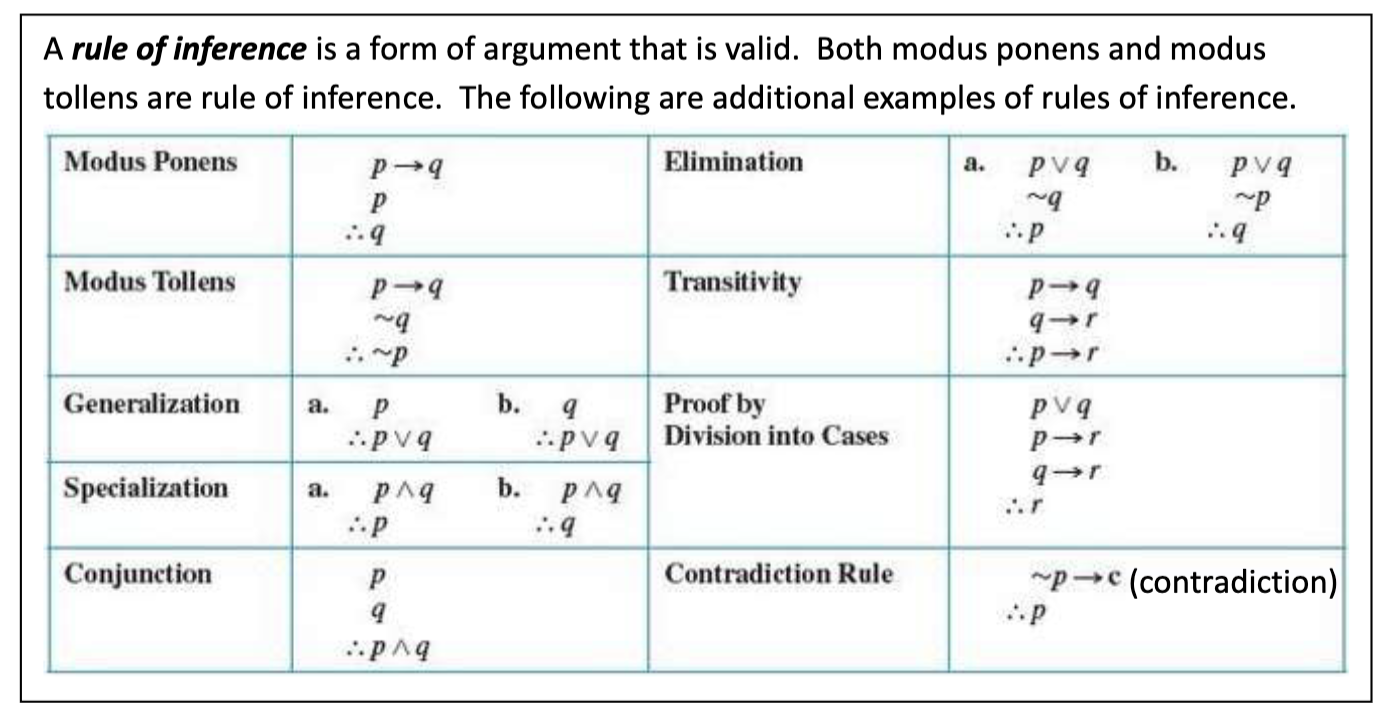
\includegraphics[width=0.75\textwidth]{rule-of-inference.png}
\end{center}

\begin{align*}
    \text{Prove by Detachment} \\
    \text{Prove by contrapositive}\\
    \text{Disjunctive of syllogism}\\
    \text{Law of Syllogism}\\
\end{align*}

\subsubsection*{Contradictions}
\paragraph*{Definition}
A contradiction is a statement that is always false.
\begin{align*}
    &\neg p \implies c\\
    &\therefore p
\end{align*}
\pagebreak
\paragraph*{2 column rule}
The 2 column rule is a way to prove by contradiction. For example with knights and knaves. Knights always
tell the truth and knaves always lie:
\begin{itemize}
    \item A says B is a knight
    \item B says A and I are of opposite types
\end{itemize}

\hrulefill\\

Suppose A is a knight:
\begin{center}
    \begin{tabular}{c|c}
    \hline
    What A says must be true & By the definition of a knight\\
    \hline
    B is a knight & by given (what A says)\\
    \hline
    What B says must be true & By the definition of a knight\\
    \hline
    A and B are of opposite types & by given (what B says)\\
    \hline
    Contradiction & A is not a knight or A is a knave\\
    \hline
    The supposition is false & by rule of contradiction\\
    \hline
    A is not a knight or A is a knave & by negation of supposition.\\
    \hline
    \end{tabular}
\end{center}

\section{The Logic of Quantified Statements}
\subsection{Predicates and Quantified Statements (Part 1)}
\hrulefill

\subsubsection*{Predicates}
\paragraph*{Definition}
A predicate is a sentence that contains a finite number of variables and becomes
a statement when specific values are substituted for the variables. For example: 
"$P(x): x$ is a positive integer" is a predicate. The statement $P(3)$ is true, while $P(-2)$ is false.

\paragraph*{Domain of a Predicate}
The Domain of a predicate is the set of all values that can be substituted for the
variable.

\paragraph*{Example}
Let $P(x)$ be the predicate "$x^2 > x$." The domain of $P(x)$ is $\mathbb{R}$.
\begin{align*}
    P(\frac{1}{2}): &\quad (\frac{1}{2})^2 > \frac{1}{2} &= False\\
    P(-\frac{1}{2}): &\quad (-\frac{1}{2})^2 > -\frac{1}{2} &= True\\
    P(2): &\quad 2^2 > 2 &= True\\
\end{align*}

\subsubsection*{Truth Sets}
\paragraph*{Definition}
If $P(x)$ is a predicate with domain $D$, the truth set of $P(x)$ is the set of all
elements in $D$ for which $P(x)$ is true when they are substituted for x. The truth 
set of $P(x)$ is denoted by:
\begin{equation*}
    \{x \in D \ni P(x)\} \subseteq D
\end{equation*}

\paragraph*{Example}
Let $P(x)$ be the predicate "$n^2 \leq 30$" with domain $\mathbb{Z}$. The truth set of $P(x)$ is:
\begin{equation*}
    \{x \in \mathbb{Z} \ni P(x)\} = \{-5, -4, -3, -2, -1, 0, 1, 2, 3, 4, 5\}
\end{equation*}

\subsubsection*{Quantified Statements}
\paragraph*{Definition}
A quantified statement is a statement that contains a quantifier. The two most common quantifiers are:
\begin{itemize}
    \item \textbf{Universal Quantifier} $\forall$ (for all)
    \item \textbf{Existential Quantifier} $\exists$ (there exists)
\end{itemize}

\paragraph*{Universal Statements}
Let $P(x)$ be a predicate with domain $D$. A univseral statment is a statement of the form 
"$\forall x \in D, P(x)$" which is read as "for all $x$ in $D$, $P(x)$ is true."
\begin{itemize}
    \item It is defined to be true if and only if $P(x)$ is true for all $x$ in $D$.
    \item It is defined to be false if and only if $P(x)$ is false for at least one $x$ in $D$.
    \item The value of $x$ for which $P(x)$ is false is called a counterexample.
\end{itemize}

\paragraph*{Example}
Let $D = \{1,2,3\}$, and show that the statement "$\forall x \in D, x^2 \geq x$" is true.
\begin{align*}
    1^2 \geq 1 &\text{ is true}\\
    2^2 \geq 2 &\text{ is true}\\
    3^2 \geq 3 &\text{ is true}\\
    \therefore \quad \forall x \in &D, x^2 \geq x \text{ is true.}
\end{align*}

\paragraph*{Existential Statements}
Let $P(x)$ be a predicate with domain $D$. An existential statement is a statement of the form
"$\exists x \in D \ni P(x)$" which is read as "there exists an $x$ in $D$ such that $P(x)$ is true."
\begin{itemize}
    \item It is defined to be true if and only if $P(x)$ is true for at least one $x$ in $D$.
    \item It is defined to be false if and only if $P(x)$ is false for all $x$ in $D$.
    \item The value of $x$ for which $P(x)$ is true is called a witness.
\end{itemize}

\paragraph*{Example}
Show that the statement "$\exists x \in \mathbb{Z} \ni \frac{1}{x} = x$" is true.
\begin{align*}
    x = 1: \frac{1}{1} &= 1 \text{ is true}\\
    \therefore \quad \exists x \in &\mathbb{Z} \ni \frac{1}{x} = x \text{ is true.}
\end{align*}

\paragraph*{Universal Conditional Statements}
A universal conditional statement is a statement of the form "$\forall x \in D, P(x) \implies Q(x)$" 
which is read as "for all $x$ in $D$, if $P(x)$ is true, then $Q(x)$ is true."


\subsection{Predicates and Quantified Statements (Part 2)}
\hrulefill

\subsubsection*{Negations of Quantified Statements}
\paragraph*{Negation of a Universal Statement}
\begin{equation*}
    \neg(\forall x \in D, P(x)) \equiv \exists x \in D \ni \neg P(x)
\end{equation*}

\paragraph*{Negation of an Existential Statement}
\begin{equation*}
    \neg(\exists x \in D \ni P(x)) \equiv \forall x \in D, \neg P(x)
\end{equation*}

\paragraph*{Negation of a Universal Conditional Statement}
\begin{equation*}
    \neg(\forall x \in D, P(x) \implies Q(x)) \equiv \exists x \in D \ni P(x) \land \neg Q(x)
\end{equation*}

Consider the statement: $\forall x \in D, P(x) \implies Q(x)$.
\begin{align*}
    \text{It's contrapositive is:} \quad &\forall x \in D, \neg Q(x) \implies \neg P(x)\\
    \text{It's converse is:} \quad &\forall x \in D, Q(x) \implies P(x)\\
    \text{It's inverse is:} \quad &\forall x \in D, \neg P(x) \implies \neg Q(x)
\end{align*}
\subsection{Statements with Multiple Quantifiers}
\hrulefill

Consider the statement: $\forall x \in D, \exists y \in E \ni P(x,y)$. To show the truth of the statement, 
we must show that for every $x$ in $D$, there exists a $y$ in $D$ such that $P(x,y)$ is true.

\paragraph*{Example}
Let $D = \{1,2,3\}$ and $P(x,y)$ be the predicate "$x + y = 4$". Show that the statement
$\forall x \in D, \exists y \in D \ni P(x,y)$ is true.
\begin{align*}
    x = 1: \quad &\exists y \in D \ni 1 + y = 4 \implies y = 3\\
    x = 2: \quad &\exists y \in D \ni 2 + y = 4 \implies y = 2\\
    x = 3: \quad &\exists y \in D \ni 3 + y = 4 \implies y = 1\\
    \therefore \quad &\forall x \in D, \exists y \in D \ni P(x,y) \text{ is true.}
\end{align*}

Consider the statement: $\exists x \in D \ni \forall y \in D, P(x,y)$. To show the truth of the statement,
we must show that there exists an $x$ in $D$ such that for every $y$ in $D$, $P(x,y)$ is true.

\paragraph*{Example}
Let $D = \{1,2,3\}$ and $P(x,y)$ be the predicate "$x + y = 4$". Show that the statement
$\exists x \in D \ni \forall y \in P, P(x,y)$ is false.
\begin{align*}
    x = 1: \quad &\forall y \in D, 1 + y = 4 \implies y = 3\\
    x = 2: \quad &\forall y \in D, 2 + y = 4 \implies y = 2\\
    x = 3: \quad &\forall y \in D, 3 + y = 4 \implies y = 1\\
    \therefore \quad &\exists x \in D \ni \forall y \in D, P(x,y) \text{ is false.}
\end{align*}

\paragraph*{Negation of Multiply-Quantified Statements}
\begin{align*}
    \neg(\forall x \in D, \exists y \in E \ni P(x,y)) &\equiv \exists x \in D \ni \forall y \in E, \neg P(x,y))\\
    \neg(\exists x \in D, \ni \forall y \in E, P(x,y)) &\equiv \forall x \in D, \exists y \in E \ni \neg P(x,y)\\
\end{align*}


\subsection{Arguments with Quantified Statements}
\hrulefill

\subsubsection*{Universal Model Ponens (Direct Proof)}
\begin{align*}
    &\forall x, P(x) \implies Q(x) \quad &\text{ If $x$ makes P(x) true, then x makes Q(x) true.}\\
    &P(a) \quad &\text{ Input $a$ makes P(a) true.}\\
    \therefore \quad &Q(a) \quad &\text{ Therefore $a$ makes Q(a) true.}
\end{align*}

\paragraph*{Example}
Let $P(x)$ be the predicate "$x$ is a prime number" and $Q(x)$ be the predicate "$x$ is an odd number".
\begin{align*}
    &\forall x, P(x) \implies Q(x) \quad &\text{If $x$ is a prime number, then $x$ is an odd number.}\\
    &P(3) \quad &\text{3 is a prime number,}\\
    \therefore \quad &Q(3) \quad &\text{therefore 3 is an odd number.}
\end{align*}

\subsubsection*{Universal Modus Tollens (Prove by Contradiction)}
\begin{align*}
    &\forall x, P(x) \implies Q(x) \quad &\text{If $x$ makes P(x) true, then $x$ makes Q(x) true.}\\
    &\neg Q(a) \quad &\text{Input $a$ makes Q(a) false.}\\
    \therefore \quad &\neg P(a) \quad &\text{Therefore $a$ does not make P(a) true.}
\end{align*}

\paragraph*{Example}
Consider the statement "All irrational numbers are real numbers.":
\begin{align*}
    &\forall x \in \mathbb{R} - \mathbb{Q}, x \in \mathbb{R} \quad &\text{If $x$ is an irrational number, then $x$ is a real number.}\\
    &\frac{1}{0} \notin \mathbb{R} \quad &\text{$\frac{1}{0}$ is not a real number,}\\
    \therefore \quad &\frac{1}{0} \notin \mathbb{R} - \mathbb{Q} \quad &\text{therefore $\frac{1}{0}$ is not an irrational number.}
\end{align*}

\subsubsection*{Converse and Inverse Errors}
\paragraph*{Converse Error}
\begin{align*}
    &\forall x, P(x) \implies Q(x)
    &Q(a)
    \therefore \quad &P(a) \text{(Invalid Arguement)}
\end{align*}

\paragraph*{Inverse Error}
\begin{align*}
    &\forall x, P(x) \implies Q(x)
    &\neg P(a)
    \therefore \quad &\neg Q(a) \text{(Invalid Arguement)}
\end{align*}

\section{Elementary Number Theory and Methods of Proof}
\subsection{Direct Proof and Counterexample}
\hrulefill

\paragraph*{Definitions}
Let P(n) be the predicate "n is an even number".
\begin{align*}
    \forall n \in \mathbb{Z}, P(n) \iff \exists k \in \mathbb{Z} \ni n = 2k.\\
    \forall n \in \mathbb{Z}, \neg P(n) \iff \exists k \in \mathbb{Z} \ni n = 2k + 1.
\end{align*}

\paragraph*{Example}
Is -301 even or odd?
\begin{align*}
    -301 &= 2k + 1 \text{ for } k=-151\\
\end{align*}

\paragraph*{Example}
If $a, b \in \mathbb{Z}$, is $6a^2b$ even?
\begin{align*}
    &\exists a, b \in \mathbb{Z} \ni 6a^2b = 2(k) + 1 \\
    &6a^2b = 2(3a^2b) \text{ for } k=3a^2b\\
    \therefore \quad &6a^2b \text{ is even.}
\end{align*}

\paragraph*{Prime and Composite Number Definition}
Let P(n) be the predicate "n is a prime number".
\begin{align*}
    \forall n \in \mathbb{Z}_{>1}, P(n) &\iff \forall r, s \in \mathbb{Z}_{>1}, n=rs \implies r=n \lor s=n\\
    \forall n \in \mathbb{Z}_{>1}, \neg P(n) &\iff \exists r, s \in \mathbb{Z}_{>1} \ni n=rs \land 1 < r < n \land 1 < s < n
\end{align*}

\subsubsection*{Constructive Proof of Existential Statement}
\begin{equation*}
    \exists x in D \ni Q(x)
\end{equation*}
\begin{itemize}
    \item Find an x in D that makes !(x) true.
    \item Give a set of directions for finding such an x in D
\end{itemize}

\paragraph*{Example}
Prove there is and even integer n such that n can be written in two ways as a sum of two prime numbers.
\begin{align*}
    \text{Let } n &= 10,\\
    10 &= 3 + 7\\
    10 &= 5+5\\
    \therefore \quad &\text{the statement is true.}
\end{align*}

\subsubsection*{Disproving Universal Statement by Counterexample}
\begin{equation*}
    \forall x in D, P(x) \implies Q(x)
\end{equation*}

\begin{itemize}
    \item Find an x in D that makes P(x) true, but Q(x) false.
\end{itemize}

% \paragraph*{Example}
% Disprove the statement $\forall n, k \in \mathbb{Z}, n = 2k \implies \frac{n-1}{2} = 2k + 1$
% \begin{align*}
%     Let n = 1\\
%     1 = 2(0) + 1, \therefore n is odd.
%     \frac{1-1}{2}
% \end{align*}

\subsubsection*{Method of Exhaustion of Proving Universal Statement}
\begin{equation*}
    \forall x in D, P(x) \implies Q(x)
\end{equation*}
\begin{itemize}
    \item Check all x in D to make sure that when P(x) is true, Q(x) is false.
\end{itemize}

% \paragraph*{Example}
% Prove the statement "$\forall n \in 4 \leq n \leq 10, n = a + b$ where a and b are prime numbers.
% \begin{align*}
%     n &= 4, \quad 4 &= 2+2
% \end{align*}

\subsubsection*{Direct Proof of Universal Statement}
\begin{equation*}
    \forall x \in D, P(x) \implies Q(x)
\end{equation*}
\begin{itemize}
    \item Suppose x is an arbitrary element in D for which the hypothesis P(x) is true.
    \item Using definitions or previously established results and rules to conclude Q(x) is true.
\end{itemize}

\paragraph*{Example}
Prove the statement "the sum of any two even integers is even."
\begin{align*}
    &\text{Suppose a and b are two even integers}\\
    \therefore \quad & a = 2k, \exists k_1 \in \mathbb{Z}\\
    \therefore \quad & b = 2k, \exists k_2 \in \mathbb{Z}\\
    \therefore \quad & a + b = 2k_1 + 2k_2\\
    \therefore \quad & a + b = 2(k_1 + k_2)\\
    \therefore \quad & a + b \text{ is even}
\end{align*}
\pagebreak
\subsection{Skipped}
\hrulefill
\subsection{Rational Numbers}
\hrulefill

\paragraph*{Definitions}
\begin{itemize}
    \item A real number r is rational if and only if $\exists a,b \in \mathbb{Z}$ such that $r = \frac{a}{b} \land b \neq 0$.
    \item A real number that is not rational is irrational.
\end{itemize}

\paragraph*{Example}
Is 320.5492492492... a rational number? (The 492 repeats). We can split the number into two parts: 320.5 and 0.0492492...
\begin{align*}
    &\text{First we rewrite 320.5 as a fraction:}\\
    & 320.5 = \frac{3205}{10}\\
    \\
    &\text{Then we rewrite 0.0492492... as a fraction:}\\
    &10000(0.0492492...) - 10(0.0492492...) = 492.492... = 0.492492... = 492\\
    \Rightarrow \quad & 10000x - 10x = 492\\
    \Rightarrow \quad & 9990x = 492\\
    \Rightarrow \quad & x = \frac{492}{9990}\\
    \\
    &\text{Now we can combine the two fractions:}\\
    & 320.5492492... = \frac{3205}{10} + \frac{492}{9990}\\
    \Rightarrow \quad & \frac{3205 \cdot 999}{10 \cdot 999} + \frac{492 \cdot 1}{9990}\\
    \Rightarrow \quad & \frac{3205 \cdot 999 + 492}{9990}\\
    \Rightarrow \quad & \frac{3199995 + 492}{9990}\\
    \Rightarrow \quad & \frac{3200487}{9990}\\
    \therefore \quad & 320.5492492... \text{ is rational.}
\end{align*}

\subsubsection*{Zero Product Property}
\paragraph*{Theorem}
If neither of two real numbers is zero, then their product is non-zero. The contrapositive of this theorem is also true: If the product of two real numbers is zero, then at least one of the two numbers is zero.
\begin{align*}
    &\text{Let } a,b \in \mathbb{Q}\\
    &\text{If } ab = 0 \Rightarrow a = 0 \lor b = 0\\
    &\text{If } ab \neq 0 \Rightarrow a \neq 0 \land b \neq 0
\end{align*}

\paragraph*{Example}
\begin{align*}
    &\text{Let } a,b \in \mathbb{Q}:\\
    \therefore \quad & a = \frac{n_1}{d_1}, \exists n_1,d_1 \in \mathbb{Z} \land d_1 \neq 0 & \text{Definition of rational numbers.}\\
    \therefore \quad & b = \frac{n_2}{d_2}, \exists n_1,d_1 \in \mathbb{Z} \land d_2 \neq 0\\
    \therefore \quad & a + b = \frac{n_1}{d_1} + \frac{n_2}{d_2} & \text{Substitution principle.}\\
    \therefore \quad & a + b = \frac{n_1d_2 + n_2d_1}{d_1d_2}\\
    \therefore \quad & d_1d_2 \neq 0 & \text{Zero product property}\\
    \therefore \quad & a + b \text{ is rational}
\end{align*}

\subsubsection*{Corollaries}
\paragraph*{Definition}
A corollary is a statement whose truth can be immediately deduced from a theorem that has already been proven.

\paragraph*{Example}
Prove that the product of two rational numbers is rational.
\begin{align*}
    &\text{Let } a,b \in \mathbb{Q}:\\
    \therefore \quad & a = \frac{n}{m}, \exists n,m \in \mathbb{Z} \land m \neq 0 & \text{Definition of rational numbers.}\\
    \therefore \quad & b = \frac{s}{t}, \exists s,t \in \mathbb{Z} \land t \neq 0\\
    \therefore \quad & a \cdot b = \frac{n}{m} \cdot \frac{s}{t}, m \neq 0 \land t \neq 0\\
    \therefore \quad & ab = \frac{ns}{mt}, mt \neq 0 & \text{Zero product property.}\\
    \therefore \quad & ab \in \mathbb{Q}
\end{align*}

\paragraph*{Example}
Prove or disprove by counterexample the following statement: "The quotient of any 2 rational numbers is rational."
\begin{align*}
    & \forall p,q \in \mathbb{Q}, \frac{p}{q} \in \mathbb{Q} & \text{Statement}\\
    & \text{Let } p=1,q=0\\
    \therefore \quad & \frac{p}{q} \notin \mathbb{Q}\\
    \therefore \quad & \exists p,q \in \mathbb{Q} \ni \frac{p}{q} \notin \mathbb{Q}
\end{align*}

\paragraph*{Example}
Prove or disprove by counterexample the following statement: $\forall a,b \in \mathbb{R}, a<b \implies a<\frac{a+b}{2}<b.$
\begin{align*}
    \therefore \quad & a < b \implies a + b < 2b\\
    \because \quad & \frac{1}{2} > 0\\
    \therefore \quad & a < b \land \frac{1}{2} > 0 \implies \frac{a+b}{2} < \frac{b}{2}\\
    \therefore \quad & a < b \implies 2a < b + a\\
    \because \quad & \frac{1}{2} > 0\\
    \therefore \quad & a < b \land \frac{1}{2} > 0 \implies a < \frac{a+b}{2}\\
    \therefore \quad & a < \frac{a+b}{2} \land \frac{a+b}{2} < b \equiv a < \frac{a+b}{2} < b\\
\end{align*}
\subsection{Divisibility}
\hrulefill

\paragraph*{Definitions}
If n and d are integers and d $\neq$ 0, then n is divisible by d if and only if n = dk for some integer k.
\begin{itemize}
    \item Notation: $d|n$ is read "d divides n".
    \begin{itemize}
        \item $d|n \iff \exists k \in \mathbb{Z} \ni n=dk$
    \end{itemize}
\end{itemize}

It is equivalent to the following statements:
\begin{itemize}
    \item n is a multiple of d
    \item d is a factor of n
    \item d is a divisor of n
    \item d divides n
\end{itemize}

\paragraph*{Example}
Prove the following statement: $\forall a,b,c \in \mathbb{Z}, a|b \land a|c \implies a|(b+c)$.
\begin{align*}
    & \text{Suppose } a,b,c \in \mathbb{Z} \land a|b \land a|c\\
    \therefore \quad & b=ak, \exists k \in \mathbb{Z} & \text{Definition of Divisibility}\\
    \therefore \quad & c=am, \exists m \in \mathbb{Z}\\
    \therefore \quad & b+c=a(k+m) & \text{Substitution and distributive}\\
    \therefore \quad & k+m \in \mathbb{Z} & \text{Integers are closed under addition}\\
    \therefore \quad & a|(b+c) & \text{Def. of divisibility}
\end{align*}

\subsubsection*{Divisibility Theorems}
\paragraph*{Positive Divisor of a Positive Integer Theorem}
\begin{equation*}
    \forall a,b \in \mathbb{Z}, a>0 \land b>0 \land a|b \implies a \leq b.
\end{equation*}

\paragraph*{Divisors of 1 Theroem}
The only divisors of 1 are 1 and -1.

\paragraph*{Transistivity of Divisibility Theorem}
\begin{equation*}
    \forall a,b,c \in \mathbb{Z}, a|b \land b|c \implies a|c
\end{equation*}

\paragraph*{Divisible by a Prime Theorem}
Any integers n > 1 is divisible by a prime number.

\paragraph*{Unique Factorization of Integers Theorem}
Given any integers n > 1, there exists k many distinct prime numbers $(p_1, \dots, p_k)$ and k many positive integers 
$(e_1, \dots, e_k)$, where k is a positive integer, such that:
\begin{equation*}
    n = \prod_{i=1}^k p_i^{e_i}
\end{equation*}

\paragraph*{Example}
If $a = \prod_{i=1}^k p_i^{e_i}$, find the standard factored form of $a^2$:
\begin{align*}
    a^2 &= \prod_{i=1}^k p_i^{e_i} \cdot \prod_{i=1}^k p_i^{e_i}\\
    &= (p_1^{e_1}p_2^{e_2} \cdots p_k^{e_k}) \cdot (p_1^{e_1}p_2^{e_2} \cdots p_k^{e_k})\\
    &= p_1^{2e_1}p_2^{2e_2} \cdots p_k^{2e_k}\\
    &= \prod_{i=1}^k p_i^{2e_i}
\end{align*}


\subsection{The Quotient-Remainder Theorem}

\paragraph*{Theorem}
\begin{equation*}
    \forall n \in \mathbb{Z}, \forall d \in \mathbb{Z}^+, \exists q,r \in \mathbb{Z} \ni n=dq+r \land 0 \leq r < d
\end{equation*}

\paragraph*{Definition}
Given any integer n and any positive integer d:
\begin{align*}
    n \div d = q\\
    n \% d = r
\end{align*}

\paragraph*{Example}
If today is tuesday, what day of the week will it be in 365 days?
\begin{equation*}
    365 \mod 7 = 1
    \text{Tuesday + 1 day} = \text{Wednesday}
\end{equation*}

\subsubsection*{The Parity Property}
\paragraph*{Definition}
We call the fact that any integer is either even or odd the parity property.
\paragraph*(Method of Proof by Division Into Cases)
To prove a statement of the form "If $A_1 or A_2 \dots or A_n$, then C."

\paragraph*{Example}
The product of two consecutive integers is even.
\begin{align*}
    & \exists n \in \mathbb{Z}\\
    \\
    & \text{Case 1: } n \text{ is even}\\
    \therefore \quad & n = 2k, \exists k \in \mathbb{Z}\\
    \therefore \quad & n + 1 = 2k + 1\\
    \therefore \quad & n(n+1) = 2k(2k+1) = \\
    \therefore \quad & n(n+1) = 2(2k^2 + k)\\
    \therefore \quad & n(n+1) \text{ is even}\\
    \\
    & \text{Case 2: } n \text{ is odd}\\
    \therefore \quad & n = 2k + 1, \exists k \in \mathbb{Z}\\
    \therefore \quad & n + 1 = 2k + 2\\
    \therefore \quad & n(n+1) = (2k + 1)(2k + 2)
    \therefore \quad & n(n+1) = 2((k + 1)(2k + 1))\\
    \therefore \quad & n(n+1) \text{ is even}
\end{align*}


\pagebreak
\subsection{Skipped}
\subsection{Contradiction and Contraposition}
\hrulefill

\subsubsection*{Method of Proof by Contradiction}
\begin{itemize}
    \item Suppose the opposite of the to-be proved conclusion.
    \item Show that this supposition leads logically to a contradiction (a statement that is always false).
    \item Conclude that the statement to be broved is true.
\end{itemize}

\paragraph*{Example}
Prove the theorem by contradiction: "There is no greatest integer."
\begin{align*}
    \text{Suppose:} \quad & \exists m \in \mathbb{Z} \ni \forall n \in \mathbb{Z}, n \leq m & \text{Opposite of theorem}\\
    \therefore \quad & \exists n \in \mathbb{Z} \ni n = m + 1\\
    \therefore \quad & \nexists m \in \mathbb{Z} \ni \forall n \in \mathbb{Z}, n \leq m\\
\end{align*}

\paragraph*{Example}
Prove the theorem by contradiction: "The square root of any irrational number is irrational."
\begin{align*}
    \text{Theorem:} \quad & \forall n \notin \mathbb{Q}, \sqrt{n} \notin \mathbb{Q} & \text{Theorem}\\
    \text{Suppose:} \quad & \forall n \notin \mathbb{Q}, \sqrt{n} \in \mathbb{Q} & \text{Opposite of theorem}\\ 
    \therefore \quad & \sqrt{n} \in \mathbb{Q} \implies \exists a, b \in \mathbb{Z} \ni \sqrt{n} = \frac{a}{b} \land b \neq 0 & \text{Definition of rational numbers}\\
    \therefore \quad & \sqrt{n} = \frac{a}{b} \implies n = \frac{a^2}{b^2} & \text{Squaring both sides}\\
    \therefore \quad & a, b \in \mathbb{Z} \implies a^2, b^2 \in \mathbb{Z} & \text{Integers are closed under squaring}\\
    \therefore \quad & n = \frac{a^2}{b^2} \land a^2, b^2 \in \mathbb{Z} \implies n \in \mathbb{Q} & \text{Definition of rational numbers}\\
    \therefore \quad & n \in \mathbb{Q} \land n \notin \mathbb{Q} & \text{Contradiction}\\
    \therefore \quad & \text{The assumption is false, and the theorem is true.}
\end{align*}

\paragraph*{Example}
Prove the theorem by contradiction: "The sum of any rational number and any irrational number is irrational."
\begin{align*}
    \text{Theorem:} \quad & \forall n \in \mathbb{Q}, \forall m \notin \mathbb{Q}, n + m \notin \mathbb{Q}\\
    \\
    \text{Suppose:} \quad & \forall n \in \mathbb{Q}, \forall m \notin \mathbb{Q}, n+m \in \mathbb{Q} & \text{Opposite of theorem}\\
    \therefore \quad & n + b \in \mathbb{Q} \implies \exists a,b \in \mathbb{Z} \ni n + m = \frac{a}{b} \land b \neq 0 & \text{Definition of rational numbers}\\
    \therefore \quad & m = \frac{a}{b} - n\\
    \therefore \quad & n \in \mathbb{Q} \implies \exists x,y \in \mathbb{Z} \ni n = \frac{x}{y} \land y \neq 0 & \text{Definition of rational numbers}\\
    \therefore \quad & m = \frac{a}{b} - \frac{x}{y}\\
    \therefore \quad & m = \frac{ay - bx}{by} \implies m \in \mathbb{Q}\\
    \therefore \quad & m \in \mathbb{Q} \land m \notin \mathbb{Q} & \text{Contradiction}\\
    \therefore \quad & \forall n \in \mathbb{Q}, \forall m \notin \mathbb{Q}, n + m \notin \mathbb{Q} & \text{The theorem is true.}
\end{align*}


\subsubsection*{Method of Proof by Contraposition}
\begin{itemize}
    \item Express the given statement in the form of "$\forall x \in D, P(x) \implies Q(x)$".
    \item Rewrite in contrapositive form: "$\forall x \in D, \neg Q(x) \implies \neg P(x)$".
    \item Prove the contrapositive by direct proof.
    \begin{itemize}
        \item Suppose $\exists x \in D \ni \neg Q(x)$.
        \item Prove $\neg P(x)$.
    \end{itemize}
\end{itemize}

\paragraph*{Example}
Prove the statement by contraposition: "For all integers m and n, if mn is even then m is even or n is even."
\begin{align*}
    \text{Theorem:} \quad & \forall m, n \in \mathbb{Z}, mn | 2 \implies m|2 \lor n|2\\
    \text{Contrapositive:} \quad & \forall m, n \in \mathbb{Z}, \neg (m|2) \land \neg(n|2) \implies \neg (mn|2)\\
    \\
    \text{Suppose:} \quad & \exists m, n \in \mathbb{Z} \ni \neg (m|2) \land \neg(n|2)\\
    \therefore \quad & \exists k, l \in \mathbb{Z} \ni m = 2k + 1 \land n = 2l + 1\\
    \therefore \quad & mn = (2k + 1)(2l + 1)\\
    \implies \quad & mn = 4kl + 2k + 2l + 1 \implies mn = 2(2kl + k + l) + 1\\
    \therefore \quad & 2kl + k + l \in \mathbb{Z} & \text{Integers are closed under addition}\\
    \therefore \quad & mn = 2(2kl + k + l) + 1 \implies \neg(mn|2)\\
\end{align*}

\section{Sequences, Induction, and Recursion}
\subsection{Sequences}
\hrulefill

\paragraph*{Definiton}
A sequence is a function whose \textbf{domain} is either all the \textbf{integers} between two given integers 
or all the integers greater than or equal to a given integers.

\paragraph*{Notation}
\begin{align*}
    a_1 &= f(1)\\
    &\cdots\\
    a_{n-1} &= f(n-1)\\
    a_n &= f(n)\\
    a_{n+1} &= f(n+1)
\end{align*}

\paragraph*{Example}
Write the first three terms of the sequence whose \textbf{explicit} or \textbf{general formula} is given:
\begin{align*}
    a_n &= \frac{(-1)^n}{2^n + 1} \text{ for } n \geq 1\\
    a_1 &= \frac{(-1)^1}{2^1 + 1} = - \frac{1}{3}\\
    a_2 &= \frac{(-1)^2}{2^2 + 1} = \frac{1}{5}\\
    a_3 &= \frac{(-1)^3}{2^3 + 1} = - \frac{1}{9}
\end{align*}

\subsubsection*{Summation Notation}
\paragraph*{Definition}
If m and n are integers andm $\leq$ n, then a \textbf{series} can be notated as:
\begin{equation*}
    \sum_{i=m}^n a_i = a_m + a_{m+1} + \cdots + a_n
\end{equation*} 

\begin{itemize}
    \item \textbf{Read as} ``the summation from i = m to n of a-sub-i''
    \item \textbf{i} is called the \mathbf{index} of the Summation
    \item \textbf{m} is called the \texbf{lower limit} of the Summation
    \item \textbf{n} is called the \texbf{upper limit} of the summation
\end{itemize}

\paragraph*{Example}
Expand and evaluate the following:
\begin{align*}
    &\sum_{i=2}^6 (i-1)^2\\
    &= 1 + 4 + 9 + 16 + 25\\
    &= 55
\end{align*}

\paragraph*{Re-indexing a Summation}
Re-indexing a summation involves changing the index variable or the limits of summation, often to simplify the expression or to match 
another sum's index.
\begin{align*}
    &\sum_{i=1}^{n+1} \frac{1}{i^2}\\
    = &\sum_{i=1}^{n} \frac{1}{i^2} + \frac{1}{(n+1)^2}
\end{align*}

\paragraph*{Example}
If $j=i+1$, transform the following summation by rewriting it in terms of j: $\sum_{i=4}^{k-1} i(i-1)$
\begin{align*}
    i &= 4 \implies j = 4 + 1 = 5 & \text{Rewrite lower limit.}\\
    i &= k - 1 \implies j = k - 1 + 1 = k & \text{Rewrite upper limit}\\
    j &= i + 1 \implies i = j - 1 & \text{Rewrite i in terms of j}\\
    & \sum_{j=5}^{k} (j-1)(j-2) & \text{Rewrite sum}
\end{align*}

\subsubsection{Product Notation}
\paragraph*{Definition}
If m and n are integers andm $\leq$ n, then a \textbf{series} can be notated as:
\begin{equation*}
    \prod_{i=m}^n a_i = a_m \cdot a_{m+1} \cdot \cdots \cdot a_n
\end{equation*} 

\begin{itemize}
    \item \textbf{Read as} ``the product from i = m to n of a-sub-i''
    \item \textbf{i} is called the \mathbf{index} of the product
    \item \textbf{m} is called the \texbf{lower limit} of the product
    \item \textbf{n} is called the \texbf{upper limit} of the product
\end{itemize}

\paragraph*{Example}
Expand and evaluate the following:
\begin{align*}
    & \prod_{k=2}^{5} \frac{k}{k+1}\\
    &= \frac{2}{2+1} \cdot \frac{3}{3+1} \cdot \frac{4}{4+1} \cdot \frac{5}{5+1}\\
    &= \frac{1}{3}
\end{align*}

\paragraph*{Theorem}
Given sequences $\{a\}$ and $\{b\}$ and $c \in \mathbb{R}$, the following equations hold:
\begin{align*}
    \sum_{i=m}^{n} a_i + \sum_{i=m}^{n} b_i &= \sum_{i=m}^{n} (a_n + b_n)\\
    c \cdot \sum_{i=m}^{n} a_i &= \sum_{i=m}^{n} c \cdot a_i\\
    \prod_{i=m}^{n} a_i \cdot \prod_{i=m}^{n} b_i &= \prod_{i=m}^{n} (a_i b_i)
\end{align*}

\paragraph*{Factorials}
\begin{equation*}
    n! = n \cdot (n-1) \cdot \dots \cdot 2 \cdot 1
\end{equation*}

\subsubsection*{Binomial Coefficient}
\paragraph*{Definition}
Let n and r be integers with $0 \leq r \leq n$, the binomial coeffecient is notated as:
\begin{equation*}
    nCr = \binom{n}{r} = \frac{n!}{r!(n-r)!}
\end{equation*}

It presents the number of combinations of choosing r items from n choices.

\paragraph*{Example}
Evaluate:
\begin{align*}
    \binom{5}{3} = \frac{5!}{3!(5-3)!} = \frac{5 \cdot 4 \cdot 3 \cdot 2 \cdot 1}{3 \cdot 2 \cdot 1 \cdot 2 \cdot 1} = \frac{5 \cdot 4}{2 \cdot 1} = 10
\end{align*}
\subsection{Mathematical Induction 1: Proving Formulas}
\hrulefill

\subsubsection*{Method of Proof by Induction}
\paragraph*{Definition}
Induction proof explores the \textbf{patterns} we recognize from a list of unknown terms.

\paragraph*{Method}
Consider the statement $\forall n \in \{a \in \mathbb{Z} : n \geq a\}, P(n)$
\begin{itemize}
    \item Step 1: \textbf{(basis step):} Show that P(a) is true.
    \item Step 2: \textbf{(inductive step):} Show that if we suppose P(k) is true, then P(k+1) is true.
\end{itemize}

\paragraph*{Example}
Use the formula to evaluate $1 + 2 + \cdots + n = \frac{n(n+1)}{2}$.
\begin{align*}
    & \text{Suppose } n = 50\\
    1 + 2 + \cdots + 50 &= \frac{50(50+1)}{2}\\
    &= \frac{50(51)}{2}\\
    &= \frac{2550}{2}\\
    &= 1275
\end{align*}


\paragraph*{Definition} If a sum with a variable number of terms is show to equal an expression that does not contain either an ellipsis 
or a summation sign, we can say that the sum is written in \textbf{closed form}.

\paragraph*{Example}
Use the formula to evaluate $1 + 2 + \cdots + n$

\subsubsection*{Geometric Series}
\paragraph*{Definition}
If $r \in \mathbb{R} \land r \neq 1$, the sum of the first n terms of a geometric series is given by:
\begin{equation*}
    \sum_{i=0}^{n} r^i = \frac{r^{n+1} - 1}{r - 1}
\end{equation*}

\paragraph*{Example}
Use the above formula to evaluate $1 + 3 + \cdots + 3^{m-2}$
\begin{align*}
    r = 3, n = m-2\\
    1 + 3 + \cdots + 3^{m-2} &= \sum_{i=0}^{m-2} 3^i\\
    &= \frac{3^{m-1} - 1}{3 - 1} = \frac{3^{m-1}-1}{2}\\
\end{align*}

\paragraph*{Example}
$3^2 + 3^3 + \cdots + 3^{m}$
\begin{align*}
   $3^2 + 3^3 + \cdots + 3^{m}$ = 1 + 3 + 3^2 + 3^3 + \cdots + 3^{m} - (1 + 3)\\
   r=3, n=m\\
\end{align*}
\subsection{Mathematical Induction 2}
\hrulefill
\subsubsection*{Deduction and Induction}
\paragraph*{Definitions}
\begin{itemize}
    \item \textbf{Deduction} is to infer a conclusion from general principles using laws of logical reasoning.
    \item \textbf{Induction} is to infer a general principle from specific examples.
\end{itemize}

\paragraph*{Example}
Use mathematical induction to prove \newline $\forall n \in \{x \in \mathbb{Z} : x \geq 0\}, 3 | (2^{2n}-1)$:
\begin{align*}
    \text{Step 0:}& \text{ Identify the property P(n)}\\
    &P(n) \equiv 3 | (2^{2n}-1)\\
    \\
    \text{Step 1:}& \text{ Prove P(0)}\\
    & 2^{2(0)} - 1 = 2^0 - 1 = 1 - 1 = 0\\
    & 3 | 0\\
    \therefore \quad & 3 | (2^{2(0)} - 1)\\
    \\
    \text{Step 2:}& \text{ Suppose P(k) is true for } k \geq 0, \text{ then prove P(k+1)}\\
    &\text{Suppose } 3 | (2^{2k} - 1)\\
    \implies& \exists m \in \mathbb{Z} \ni 2^{2k} - 1 = 3m\\
    \implies& 2^{2(k+1)}-1 = 2^{2k} \cdot 2^{2} - 1\\
    \implies& 2^{2(k+1)}-1 = 4 \cdot 2^{2k} - 1\\
    \implies& 2^{2(k+1)}-1 = 4(2^{2k} - 1) + 3\\
    \implies& 2^{2(k+1)}-1 = 4(3m) + 3\\
    \therefore \quad & 3 | (2^{2(k+1)} - 1)\\
\end{align*}

\paragraph*{Example}
Use mathematical induction to prove \newline $\forall n \in \{x \in \mathbb{Z} : x \geq 5\}, n^2 < 2^n$
\begin{align*}
    &\text{Base Step: } n = 5\\
    &\quad 5^2 < 2^5 = 25 < 32\\
    \\
    &\text{Inductive Step:} \text{ Suppose } \forall k \in \{x \in \mathbb{Z} : x \geq 5\}, k^2 < 2^k \text{ then prove } (k+1)^2 < 2^{k+1}\\
    &\quad \text{LHS} = (k+1)^2\\
    &\qquad (k+1)^2 = k^2 + 2k + 1\\
    &\qquad k^2 < 2^k \implies k^2 + 2k + 1 < 2^k + [2k + 1]\\
    \\
    &\quad \text{RHS} = 2^{k+1}\\
    &\qquad 2^{k+1} = 2^k \cdot 2^1 = 2^k + [2^k]\\
    \\
    &\quad \text{Prove } (k+1)^2 < 2^{k+1} \text{ for } k \geq 5:\\
    &\qquad 2 \cdot 5 + 1 = 11 < 32 = 2^5\\
    &\qquad 2 \cdot 6 + 1 = 13 < 64 = 2^6\\
    &\qquad 2 \cdot 7 + 1 = 15 < 128 = 2^7\\
    &\qquad \text{and so on.}\\
    &\quad \therefore \quad \forall k \in \{x \in \mathbb{Z} : x \geq 5\}, 2k+1 < 2^k\\
    \\
    &\quad \therefore \quad \forall k \in \{x \in \mathbb{Z} : x \geq 5\}, (k+1)^2 < 2^{k+1}\\
    &\quad \therefore \quad \forall k \in \{x \in \mathbb{Z} : x \geq 5\}, k^2 < 2^k
\end{align*}

\subsubsection*{Recursion}
\paragraph*{Definition}
A \textbf{recursion} is a function that is defined in terms of itself. A recursive function is a function that calls itself.
\paragraph*{Example}
$a_k = 5a_{k-1}$ for all integers $k \geq 2$.

\subsection{Strong Mathematical Induction}
\hrulefill

\subsubsection*{Principle of Strong Mathematical Induction}
Let P(n) be a property that is defined for integers n, and let a and b be fixed integers with $a \leq b$.
\begin{itemize}
    \item Basis Step: Show that P(a), P(a+1), \dots, P(b) are all true.
    \item Inductive Step: Show that for every ingeger $k \geq b$, if P(a), P(a+1), \dots, P(k) are all true, then P(k+1) is true.
\end{itemize}

\paragraph*{Example}
Prove that $S_n = 5^n - 1 \forall n \in \mathbb{Z}^+$ if $S_0 = 0$, $S_1 = 4$, $S_k = 6S_{k-1} - S_{k-2}$ for all integers $k \geq 2$.
\begin{align*}
    \text{Basic step:}&\\
    &S_0 = 5^0 - 1 = 1 - 1 = 0\\
    &S_1 = 5^1 - 1 = 5 - 1 = 4\\
    \text{Inductive step:}&\\
    %Finish this
\end{align*}


\subsection{Skipped}
\pagebreak
\include{chapter-5/6-recursive-definition-of-sequences.tex}
\subsection{Solving Recurrence relations by Iteration}
\hrulefill\\
\paragraph*{Method}
Starting from the initial conditions, calculate the successive terms of sequences from the recurrence formula until a pattern emerges. 
Then, use the pattern to find a closed form for the sequence.

\paragraph*{Example}
\begin{equation*}
    a_n =
    \begin{cases}
        1, & n = 0\\
        a_{n-1} + 2, & \forall n \in \mathbb{Z}^+\\
    \end{cases}
\end{equation*}
Solve the recurrence relation.
\begin{align*}
    \forall n \in \mathbb{Z}^+, a_k = a_{k-1} + 2\\
    a_n = (a_{n-1} + 2) + 2\\
    a_n = (a_{n-2} + 2) + 2(2)\\
    \cdots\\
    a_n = a_{n-k} + k(2)\\
    \therefore \quad \forall n \in \mathbb{Z}^+, \quad a_n = a_0 + 2n\\
    \therefore \quad \forall n \in \mathbb{Z}^+, \quad a_n = 1 + 2n
\end{align*}

\subsubsection*{Arithmetic Sequence}
\paragraph*{Definition}
A sequence is arithmetic if there is a constant $d$ such that:
\begin{equation*}
    \forall k \in \mathbb{Z}^+, \quad  a_k = a_{k-1} + d
\end{equation*}
\paragraph*{General Formula}
\begin{equation*}
    \forall n \in \{x \in \mathbb{Z} : x \geq 0\}, \quad a_n = a_0 + nd
\end{equation*}

\subsubsection*{Geometric Sequence}
\paragraph*{Definition}
A sequence is geometric if there is a constant $r$ such that:
\begin{equation*}
    \forall k \in \mathbb{Z}^+, \quad  a_k = a_{k-1}r
\end{equation*}
\paragraph*{General Formula}
\begin{equation*}
    \forall n \in \{x \in \mathbb{Z} : x \geq 0\}, \quad a_n = a_0 r^n
\end{equation*}

\paragraph*{Example}
Use iteration to find the explicit formula of the following sequence:
\begin{equation*}
    e_k = 
    \begin{cases}
        2, & k = 0\\
        4e_{k-1} + 5, & k \geq 0
    \end{cases}
\end{equation*}

\begin{align*}
    e_0 &= 2\\
    e_1 &= 4(2) + 5\\
    e_2 &= 4(4(2) + 5) + 5 = 4^2(2) + 4(5) + 5\\
    e_3 &= 4(4^2(2) + 4(5) + 5) + 5 = 4^3(2) + 4^2(5) + 4(5) + 5\\
    &\cdots\\
    e_k &= 4^k(2) + 4^{k-1}(5) + 4^{k-2}(5) + \cdots + 4(5) + 5\\
    &= 4^k(2) + 5 \sum_{i=0}^{k-1} 4^i = 4^k(2) + 5 (\frac{4^{k-1+1} - 1}{4 - 1})\\
    e_k &= 4^k(2) + 5 (\frac{4^{k} - 1}{3})
\end{align*}

\section{Chapter 6}
\subsection{Set Theory}
\hrulefill\\

\subsubsection*{Definitions}
\begin{align*}
    A \subseteq B &\iff \forall x \in A \implies x \in B\\
    A \nsubseteq B &\iff \exists x \in A \implies x \neq B\\
\end{align*}

A is a \textbf{proper subset} of B ($A \subset B$) if and only if:
\begin{itemize}
    \item $A \subseteq B$ and
    \item $\exists x$ such that $x \in B$ and $x \notin A$
\end{itemize}

\paragraph*{Example}
Let 
\begin{align*}
    A &= \{m \in \mathbb{Z} | \exists r \in \mathbb{Z} \ni m = 6r + 12\}\\
    B &= \{n \in \mathbb{Z} | \exists s \in \mathbb{Z} \ni n = 3s\}\\
    \\
    A \subseteq B?:\\
    &6r + 12 = 6(r + 2) \implies A = \{m \in \mathbb{Z} | \exists t \in \mathbb{Z} \ni m = 6t\}\\
    &m = 6n \implies m = 3(2n)\\
    \therefore \quad & A \subseteq B\\
\end{align*}

\subsubsection*{Set Equivalence}
\paragraph*{Definition}
Given sets A and B:
\begin{equation}
    A = B \iff A \subseteq B \land B \subseteq A
\end{equation}

\paragraph*{Example}
Let
\begin{align*}
    R &= \{x \in \mathbb{Z} : 2|x\}\\
    T &= \{x \in \mathbb{Z} : 6|x\}\\
    \\
    R \subseteq T &\equiv \text{False}\\
    & Let x \in R and x = 2(1) = 2, \text{ but } 2 \neq 6k \forall k \in \mathbb{Z}\\
    \implies \quad & x \notin T\\
    \therefore \quad & R \nsubseteq T\\
    \\
    T \subseteq R &\equiv \text{True}\\
    \therefore \quad & R \neq T\\
    & Let x \in T\\
    \implies \quad & \exists k \in \mathbb{Z} \ni x = 6k \implies x = 2(3k)\\
    \implies \quad & 3k \in \mathbb{Z} \implies 2 | x \implies x \in R\\
    \therefore \quad & T \subseteq{R}
\end{align*}

\begin{center}
    \includegraphics*[width=\textwidth]{venn-diagrams.png}\\
    \includegraphics*[width=\textwidth]{set-operations.png}
\end{center}

\paragraph*{Example}
Let 
\begin{align*}
    U &= \{1, 2, 3, 4, 5, 6, 7\}\\
    A &= \{1, 3, 5, 7\}\\
    B &= \{4, 5, 6, 7\}\\
    \\
    A \cup B &= \{1, 3, 4, 5, 6, 7\}\\
    A \cap B &= \{5, 7\}\\
    B - A &= \{4, 6\}\\
    A^c &= \{2, 4, 6\}
\end{align*}

\subsubsection*{Interval Notation}
\includegraphics*[width=\textwidth]{interval-notation.png}

\paragraph*{Example}
Let $U = \mathbb{R}$,$A = (-1, 0]$ and $B = [0, 1)$
\begin{align*}
    A \cup B &= \{-1, 1\}\\
    A \cap B &= \{0\}\\
    B - A &= (0, 1)\\
    A^c &= (- \infty, 1] \cup (0, \infty)
\end{align*}

\subsubsection*{Disjoint Sets}
\paragraph*{Definition}
\begin{center}
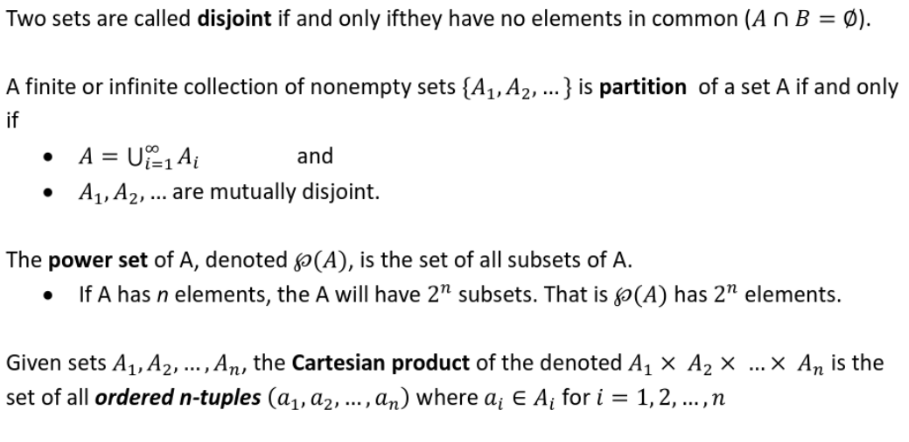
\includegraphics[width=\textwidth]{disjoint-sets.png}    
\end{center}


\paragraph*{Example}
Find $\mathcal{P}(A)$ if $A = \{1,2\}$
\begin{align*}
    \mathcal{P}(A) = \{\varnothing, 1, 2, (1,2)\}
\end{align*}
\pagebreak

\section{Chapter 7}

\end{document}